\documentclass[a4paper,12pt]{article}

% Packages for formatting
\usepackage[margin=2.5cm]{geometry} % Adjust margins
\usepackage{setspace} % Adjust line spacing
\usepackage{parskip} % Remove paragraph indentation
\usepackage{titlesec} % Customize section headings
\usepackage{lipsum} % For generating dummy text
\usepackage{graphicx}
\usepackage{float}
\usepackage{hyperref}

% Title and author
\title{pRES in the field 101}
\author{Written by: Reza Ershadi}
\date{\today}

% Section headings formatting
\titleformat{\section}{\normalfont\bfseries}{\thesection}{1em}{}
\titlespacing*{\section}{0pt}{\baselineskip}{0.5\baselineskip}

% Set line spacing
\onehalfspacing

\begin{document}

\maketitle

\section{Introduction}
This report presents a concise field protocol for the phase-sensitive Radio Echo Sounder (pRES)
system, specifically tailored for data collection on ice and glaciers. The protocol outlines the
correct setup procedures for the radar and antenna, as well as provides code snippets for assessing
data quality and conducting quick ice fabric analysis. By following this protocol, the collection of
pRES data within the ice community will become more coherent and accessible for analysis across
various applications.

\section{Field Setup: Antenna and Radar Configuration}
When conducting pRES measurements, a minimum configuration consists of one transmitting (Tx) antenna
and one receiving (Rx) antenna. However, for studying ice fabric, data collection in quad-pol mode
is necessary. This requires a convenient four-antenna setup known as Multiple-Input Multiple-Output
(MIMO). Nonetheless, it is still possible to measure quad-pol data using only two antennas by
rotating them between measurements. This section provides instructions on setting up the pRES system
with both two and four antennas, ensuring accurate data collection.


\subsection{The Importance of Field Documentation}
When collecting pRES data, meticulous documentation of all relevant details is crucial for accurate
analysis and interpretation. Even if the antenna setup deviates from the recommended protocol,
having comprehensive documentation allows for post-processing corrections. It is essential to record
several key parameters in your field notebook, including:

\begin{itemize}
\item \textbf{Distance between antennas:} The distance between antennas is a critical factor that
affects the quality and resolution of the collected data. While the specific distance may vary based
on the available cable length, a distance of around 8 meters is generally recommended. However, you
can adjust the distance to be shorter (minimum 2 meters), ensuring that the Tx and Rx antennas are
not placed right next to each other.

\item \textbf{Azimuthal orientation:} The azimuthal orientation of the antennas plays a significant
role in capturing the georeferenced ice fabric orientation. It is recommended to position the
antennas in a way that the aerial line connecting the Tx and Rx aligns with the flow direction.

\item \textbf{Antenna orientation:} The orientation of the antennas should be clearly defined based
on the direction of the cable emanating from each antenna. This information ensures consistency and
aids in the correct interpretation of the data during post-processing and analysis.

\end{itemize}

\subsection{Setting up the pRES System}
This subsection provides step-by-step instructions for setting up the pRES system, covering both the
two-antenna and four-antenna configurations. By following these guidelines, users can ensure
accurate data collection and facilitate subsequent analysis.

\subsubsection{Two-Antenna Setup}
To collect quad-pol data with two antennas, you need to perform at least 3 measurements. The 4th
measurement is optional and serves as a safety measure, as two of the measurements should be
identical if the antennas are set up correctly. It is highly recommended to name your pRES.dat files
based on the antenna orientation. A suggested naming convention is $X_{TX}X_{RX}$\_$Y_{TX}Y_{RX}$,
where "X" represents the orientation of the electric field in the antenna (H for horizontal, V for
vertical), and "Y" specifies the orientation of the cable coming out of the antenna relative to the
position of the operator (L for left, R for right, U for up, D for down). This naming convention
aids in correcting the sign of the data by applying a minus factor during post-processing.

It is easier to start with the HH orientation. The cable orientation is flexible, but it is
recommended to begin with RR as shown in Figure \ref{fig:HHRR} and collect the HH\_RR data.

\begin{figure}[H]
    \centering
    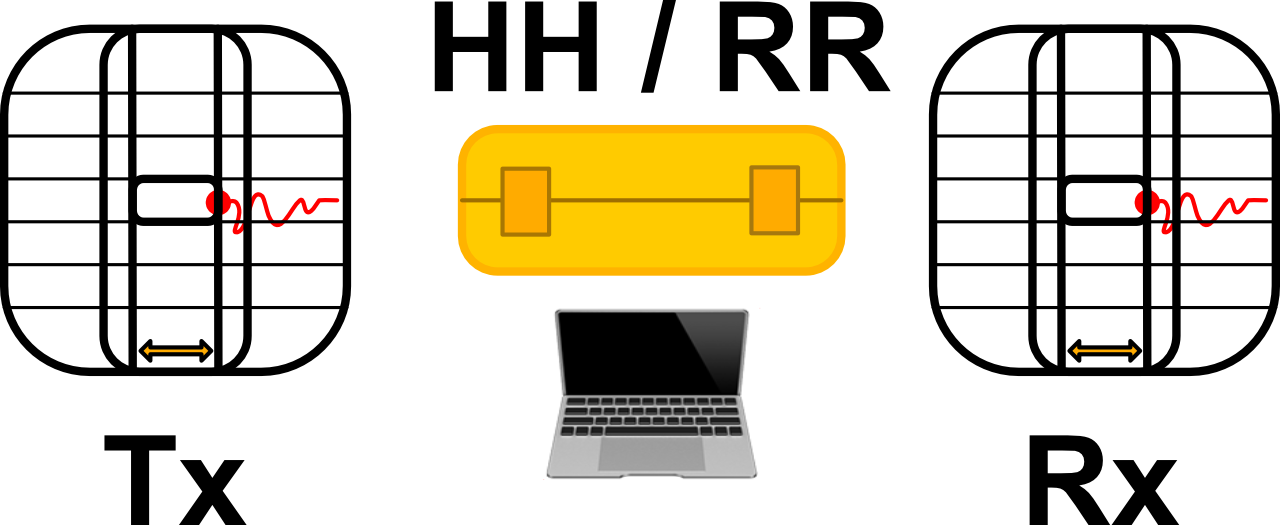
\includegraphics[width=0.8\textwidth]{figures/HHRR.png}
    \caption{Two-antenna setup in HH\_RR, with the operator and pRES system in the center. 
    The yellow two-sided arrow indicates the direction of the electric field in the antenna, and the red line represents the cable.}
    \label{fig:HHRR}
\end{figure}

The next step is to rotate the Rx antenna 90 degrees counterclockwise, as shown in Figure
\ref{fig:HVRU}, and collect the HV\_RU data.

\begin{figure}[H]
    \centering
    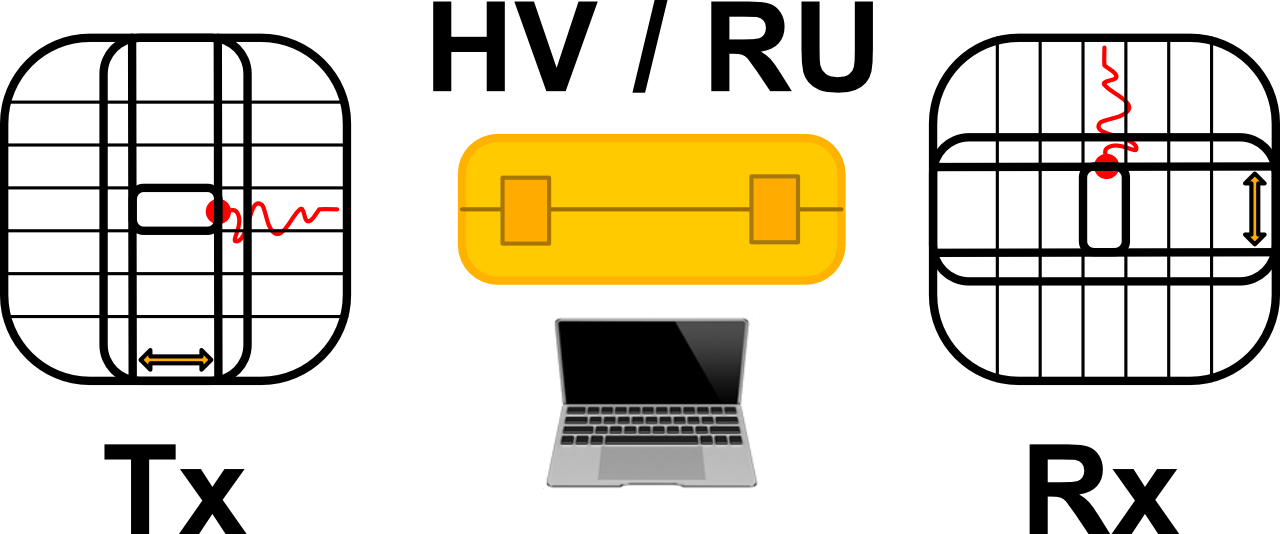
\includegraphics[width=0.8\textwidth]{figures/HVRU.png}
    \caption{Two-antenna setup in HV\_RU, with the operator and pRES system in the center.}
    \label{fig:HVRU}
\end{figure}

Then, rotate the Tx antenna 90 degrees counterclockwise, as shown in Figure \ref{fig:VVUU}, and
collect the VV\_UU data.

\begin{figure}[H]
    \centering
    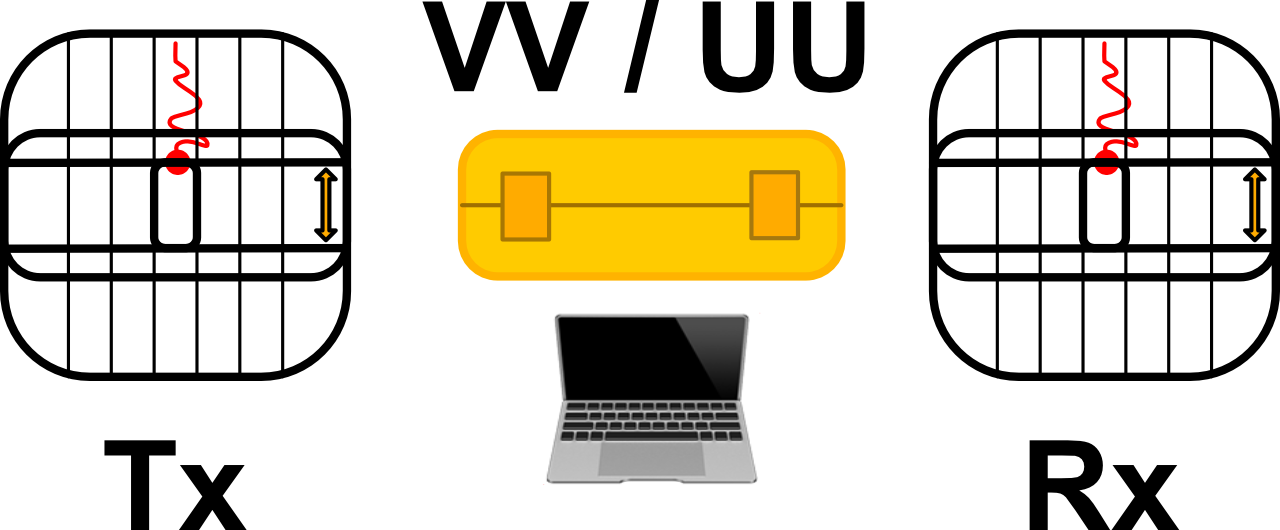
\includegraphics[width=0.8\textwidth]{figures/VVUU.png}
    \caption{Two-antenna setup in VV\_UU, with the operator and pRES system in the center.}
    \label{fig:VVUU}
\end{figure}

To complete the data collection for ice fabric analysis, you can optionally perform VH\_UR
measurements by rotating the Rx antenna 90 degrees clockwise, as shown in Figure \ref{fig:VHUR}.
However, if the antennas are positioned correctly, HV\_RU and VH\_UR measurements should be identical,
making this step optional.

\begin{figure}[H]
    \centering
    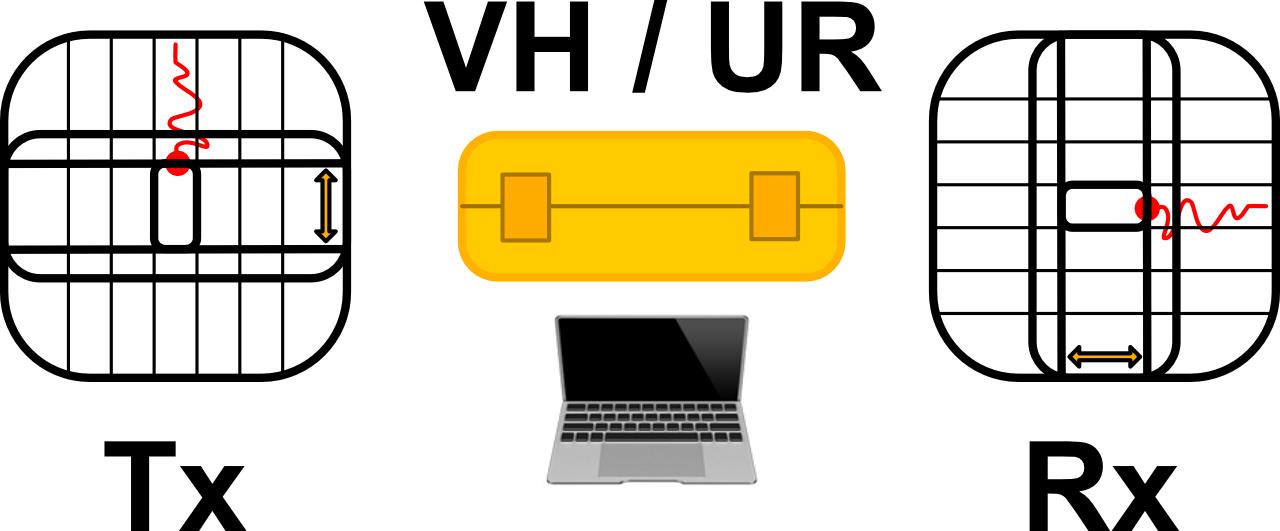
\includegraphics[width=0.8\textwidth]{figures/VHUR.png}
    \caption{Two-antenna setup in VH\_UR, with the operator and pRES system in the center.}
    \label{fig:VHUR}
\end{figure}

\subsubsection{Four-Antenna (MIMO) Setup}
If you have a multichannel pRES with four antennas, collecting quad-pol data becomes significantly
easier, faster, and less prone to errors because no antenna rotation is required. In this method,
you need to set up two Tx antennas and two Rx antennas in a line, as depicted in Figure
\ref{fig:MIMO}. It is important to note that the orientation of the Tx antennas differs: one is in
the horizontal (H) direction, while the other is in the vertical (V) direction. The same principle
applies to the Rx antennas.

\begin{figure}[h!]
\centering
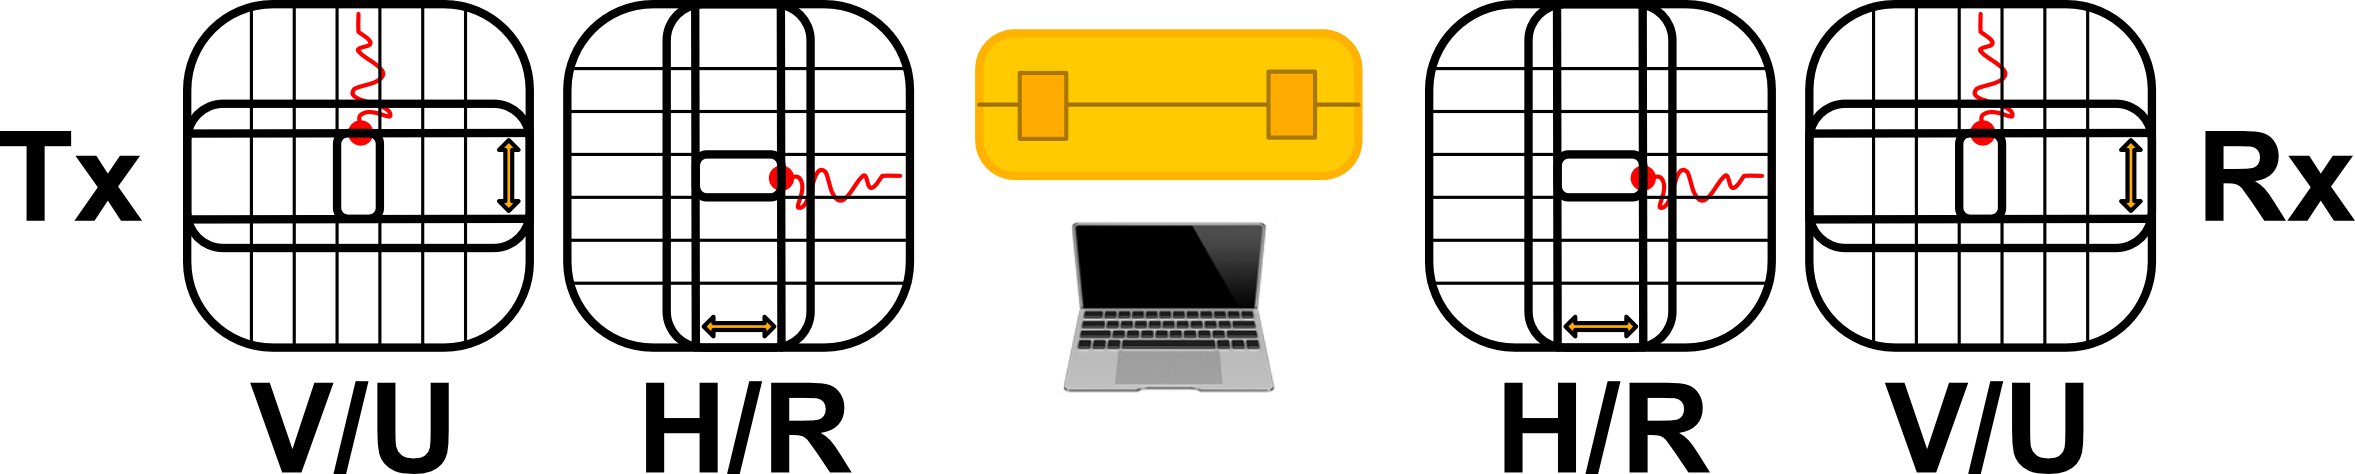
\includegraphics[width=0.8\textwidth]{figures/MIMO.png}
\caption{Four-antenna setup (MIMO) with the operator and pRES system in the center.}
\label{fig:MIMO}
\end{figure}

\subsection{pRES HTML UI}
I highly recommend reading the pRES manual for detailed instructions on how to record data using
your computer and Ethernet cable after positioning your antenna. However, here are a few important
points to consider:

\begin{itemize}
\item Ensure that the time is synchronized.
\item Select the correct antenna ports.
\item Choose the appropriate attenuator and gain settings (these depend on the ice properties and
thickness, so you may need to experiment with different values - refer to the pRES manual).
\item Select a reasonable number of sub-bursts (at least 10).
\item Remember to give your file a proper name, following the XX\_YY naming convention.
\end{itemize}

\section{How to Check Data}
The provided source code in this package, except for the fmcw functions, was written by me.
Therefore, if you encounter any issues, feel free to reach out to me directly. Please note that the
"findbed" function was recently developed by me, and there may be cases where it fails. Please keep
this in mind.

\subsection{Test Data}
To facilitate code verification and visualization, I have included two different data sets. The
first data set consists of measurements from two antennas, resulting in four individual
mono\_XX\_YY.dat files. The second data set is a MIMO file that combines all four measurements into a
single file.

\subsection{Checking the Signal}
The "BurstCheck.m" MATLAB script can help you assess the quality of an individual $*.dat$ file
recorded in the field. It quickly provides information about ice thickness and whether voltage
clipping is occurring.

\subsection{Checking the Fabric}
The "FabricCheck.m" script plots all the metrics required to evaluate the ice fabric. Before running
it, make sure to review the input parameters section in the code. Note that the MONO test data files
are recorded with the correct antenna orientation, so no minus correction is needed. However, the
MIMO test file requires a minus correction, which is applied in the code. If you follow the protocol
explained here for data collection, make sure to set all the correction factors to one.

\end{document}
